\documentclass[10pt,twocolumn,letterpaper]{article}

% --- Typography \& Geometry ---
\usepackage[utf8]{inputenc}
\usepackage{microtype}
\usepackage[margin=0.75in,top=0.85in,bottom=0.85in]{geometry}

% --- Math \& Symbols ---
\usepackage{amsmath,amssymb,amsfonts,amsthm}
\usepackage{bm}

% --- Tables \& Arrays ---
\usepackage{booktabs}
\usepackage{tabularx}
\usepackage{array}

% --- Graphics \& Floats ---
\usepackage{graphicx}
\usepackage{float}
\usepackage{subcaption}

% --- Code Listings ---
\usepackage{xcolor}
\usepackage{listings}

\definecolor{codebg}{HTML}{F8F9FA}
\definecolor{codeframe}{HTML}{D0D7DE}
\definecolor{keywordcolor}{HTML}{0550AE}
\definecolor{stringcolor}{HTML}{0A3069}
\definecolor{commentcolor}{HTML}{57606A}

\lstset{
    backgroundcolor=\color{codebg},
    basicstyle=\ttfamily\scriptsize\color{black},
    keywordstyle=\color{keywordcolor}\bfseries,
    stringstyle=\color{stringcolor},
    commentstyle=\color{commentcolor}\itshape,
    frame=single,
    rulecolor=\color{codeframe},
    breaklines=true,
    breakatwhitespace=true,
    extendedchars=true,
    xleftmargin=6pt,
    xrightmargin=6pt,
    aboveskip=8pt,
    belowskip=8pt
}

% --- Hyperlinks ---
\usepackage{hyperref}
\hypersetup{
    colorlinks=true,
    linkcolor=blue!70!black,
    citecolor=blue!70!black,
    urlcolor=blue!70!black
}

% --- Input Title \& Authors ---
% Metadata for block_transformer_hiba
\title{\textbf{Hierarchical Intra-Block and Inter-Block Attention (HIBA): Efficient Block-Sparse Attention with Periodic Dense Rectification}}

\author{
  \textbf{Taha Majs}\thanks{Corresponding author: tahamajs@uni.edu} \quad \textbf{Research Team} \\
  Department of Computer Science \\
  Advanced Machine Learning \& Efficiency Laboratory
}

\date{\today}


\begin{document}

\maketitle

% --- Abstract \& Keywords Block ---
\begin{abstract}
Transformer self-attention scales quadratically with sequence length, making long-context inference prohibitively expensive on memory-constrained hardware. Existing sparse approaches trade accuracy for efficiency by permanently discarding tokens, which degrades performance on tasks requiring global reasoning. We introduce \textbf{Hierarchical Intra-Block and Inter-Block Attention (HIBA)}, a block-sparse hybrid attention mechanism that strictly bounds memory scaling while maintaining global context routing.

HIBA divides the sequence into chunks of size $W$, computing exact dense attention intra-block and sparse Top-K attention inter-block. To prevent information bottlenecking, HIBA employs a periodic dense rectification strategy, falling back to exact full attention every $k$ layers. We transfer base weights exactly from pretrained attention modules via a robust extraction procedure supporting flat (DistilBERT), nested (RoBERTa), and causal fused (GPT-2) architectures. Trainable capacity is provided through residual LoRA adapters initialized to zero, allowing the mechanism to adapt without catastrophic forgetting.

We evaluate on DistilBERT, RoBERTa-base, and GPT-2 on the SST-2 sentiment task with 50 LoRA recovery steps at rank 16. HIBA achieves \textbf{90.35\%} on DistilBERT ($\Delta$ = -0.36), \textbf{78.40\%} on RoBERTa ($\Delta$ = -0.16), and \textbf{79.10\%} on GPT-2 ($\Delta$ = -0.26). Parameter count changes by \textbf{+0.89\%} due to residual LoRA adapters. Peak inference VRAM decreases by \textbf{-35\%} on long sequences, though wall-clock latency currently increases by \textbf{1.2$\times$} due to Python loop overhead in inter-block sparse indexing. Our results demonstrate that periodic rectification successfully stabilizes sparse transformers across diverse architectural families.

\textbf{Keywords:} efficient attention, block-sparse attention, LoRA, KV-cache, transformer compression




\vspace{0.5em}
\noindent\textbf{Keywords:} efficient attention, block-sparse attention, LoRA, KV-cache, transformer compression
\end{abstract}

\vspace{1em}

% --- Paper Body ---
\textit{(                                               HIBA)}

\begin{lstlisting}
# 1. Introduction

## 1.1 Motivation

Standard scaled dot-product attention (Vaswani et al., 2017) computes the attention matrix at $\mathcal{O}(L^2)$ time and memory complexity. While sparse attention patterns (such as Longformer and BigBird) reduce this to $\mathcal{O}(L \sqrt{L})$ or $\mathcal{O}(L)$, they permanently sever global token-to-token routing pathways. This strict sparsity often causes catastrophic accuracy degradation when injected post-training into dense models. 

## 1.2 Problem Statement

Given a pretrained transformer $\mathcal{M}$, we seek a modified attention function $\mathcal{A}'$ that replaces $\mathcal{A}$ such that memory scales sub-quadratically, yet global context is not permanently lost. We impose the constraints:
1. **No retraining of base weights.** 
2. **Robust architectural support.** Must seamlessly handle nested encoders (RoBERTa), fused weights (GPT-2), and modern features like GQA and RoPE without double-projection errors.

## 1.3 Our Approach

We propose **Hierarchical Intra-Block and Inter-Block Attention (HIBA)**. HIBA processes tokens in local blocks (e.g., $B=64$) for precise local semantics. For global context, it sparsely attends to a dynamic Top-K subset of tokens from neighboring blocks. Most critically, to prevent the "lost in the middle" degradation inherent to sparse architectures, HIBA employs **Periodic Dense Rectification**, executing a full $\mathcal{O}(L^2)$ attention pass at a configurable interval (e.g., every 4th layer). 

\end{lstlisting}


\section{02 Related}

Draft content for block_transformer_hiba.

\section{03 Background}

Draft content for block_transformer_hiba.

\section{04 Method}

Draft content for block_transformer_hiba.

\textit{(                                                                                )}

\begin{lstlisting}
# 5. Architecture Integration

A major contribution of HIBA is its robust `copy_weights` procedure, designed to seamlessly inject into disparate transformer families without silent failures.

## 5.1 Nested Encoder Detection (RoBERTa / BERT)

RoBERTa's attention block wraps the self-attention mechanism in an outer `BertSelfOutput` class that applies the final dense projection:

\end{lstlisting}
\section{HIBA Auto-Detection Logic}
if hasattr(pretrained\_attn, "self") and hasattr(pretrained\_attn.self, "query"):
    self.is\_nested\_encoder = True

\begin{lstlisting}

When `is_nested_encoder` is True, HIBA intercepts the forward pass *before* `self.out_proj` is applied, preventing severe signal attenuation caused by double-projection. The base weights for `W_q, W_k, W_v` are extracted deeply from `pretrained_attn.self`.

## 5.2 Fused Conv1D Handling (GPT-2)

GPT-2 stores $Q,K,V$ weights as a single fused `Conv1D` tensor with transposed dimensions $(d, 3d)$. HIBA detects this, transposes the weights to standard linear layout $(3d, d)$, and strictly chunks them:

\end{lstlisting}
c\_w = c\_w.t()
split\_size = c\_w.size(0) // 3
extracted["q"] = c\_w[:split\_size, :]
extracted["k"] = c\_w[split\_size : 2 * split\_size, :]
\section{...}

\begin{lstlisting}

## 5.3 Modern Architectural Features

* **Grouped-Query Attention (GQA):** HIBA natively checks if `num_kv_heads < num_heads` and dynamically applies `repeat_kv` during the forward pass, ensuring compatibility with Qwen, LLaMA, and Mistral.
* **Rotary Position Embeddings (RoPE):** HIBA implements `apply_rotary_pos_emb` with partial dimension rotation. It rotates only the first `rotary_dim` coordinates and concatenates the unrotated pass-through coordinates, perfectly matching Qwen3.5's behavior (e.g., `head_dim=256, rotary_dim=64`).
* **Strict Causality:** Causal masks are natively applied in both intra-block, inter-block, and rectification branches if `is_decoder=True`.

\end{lstlisting}



\begin{figure}[H]
\centering
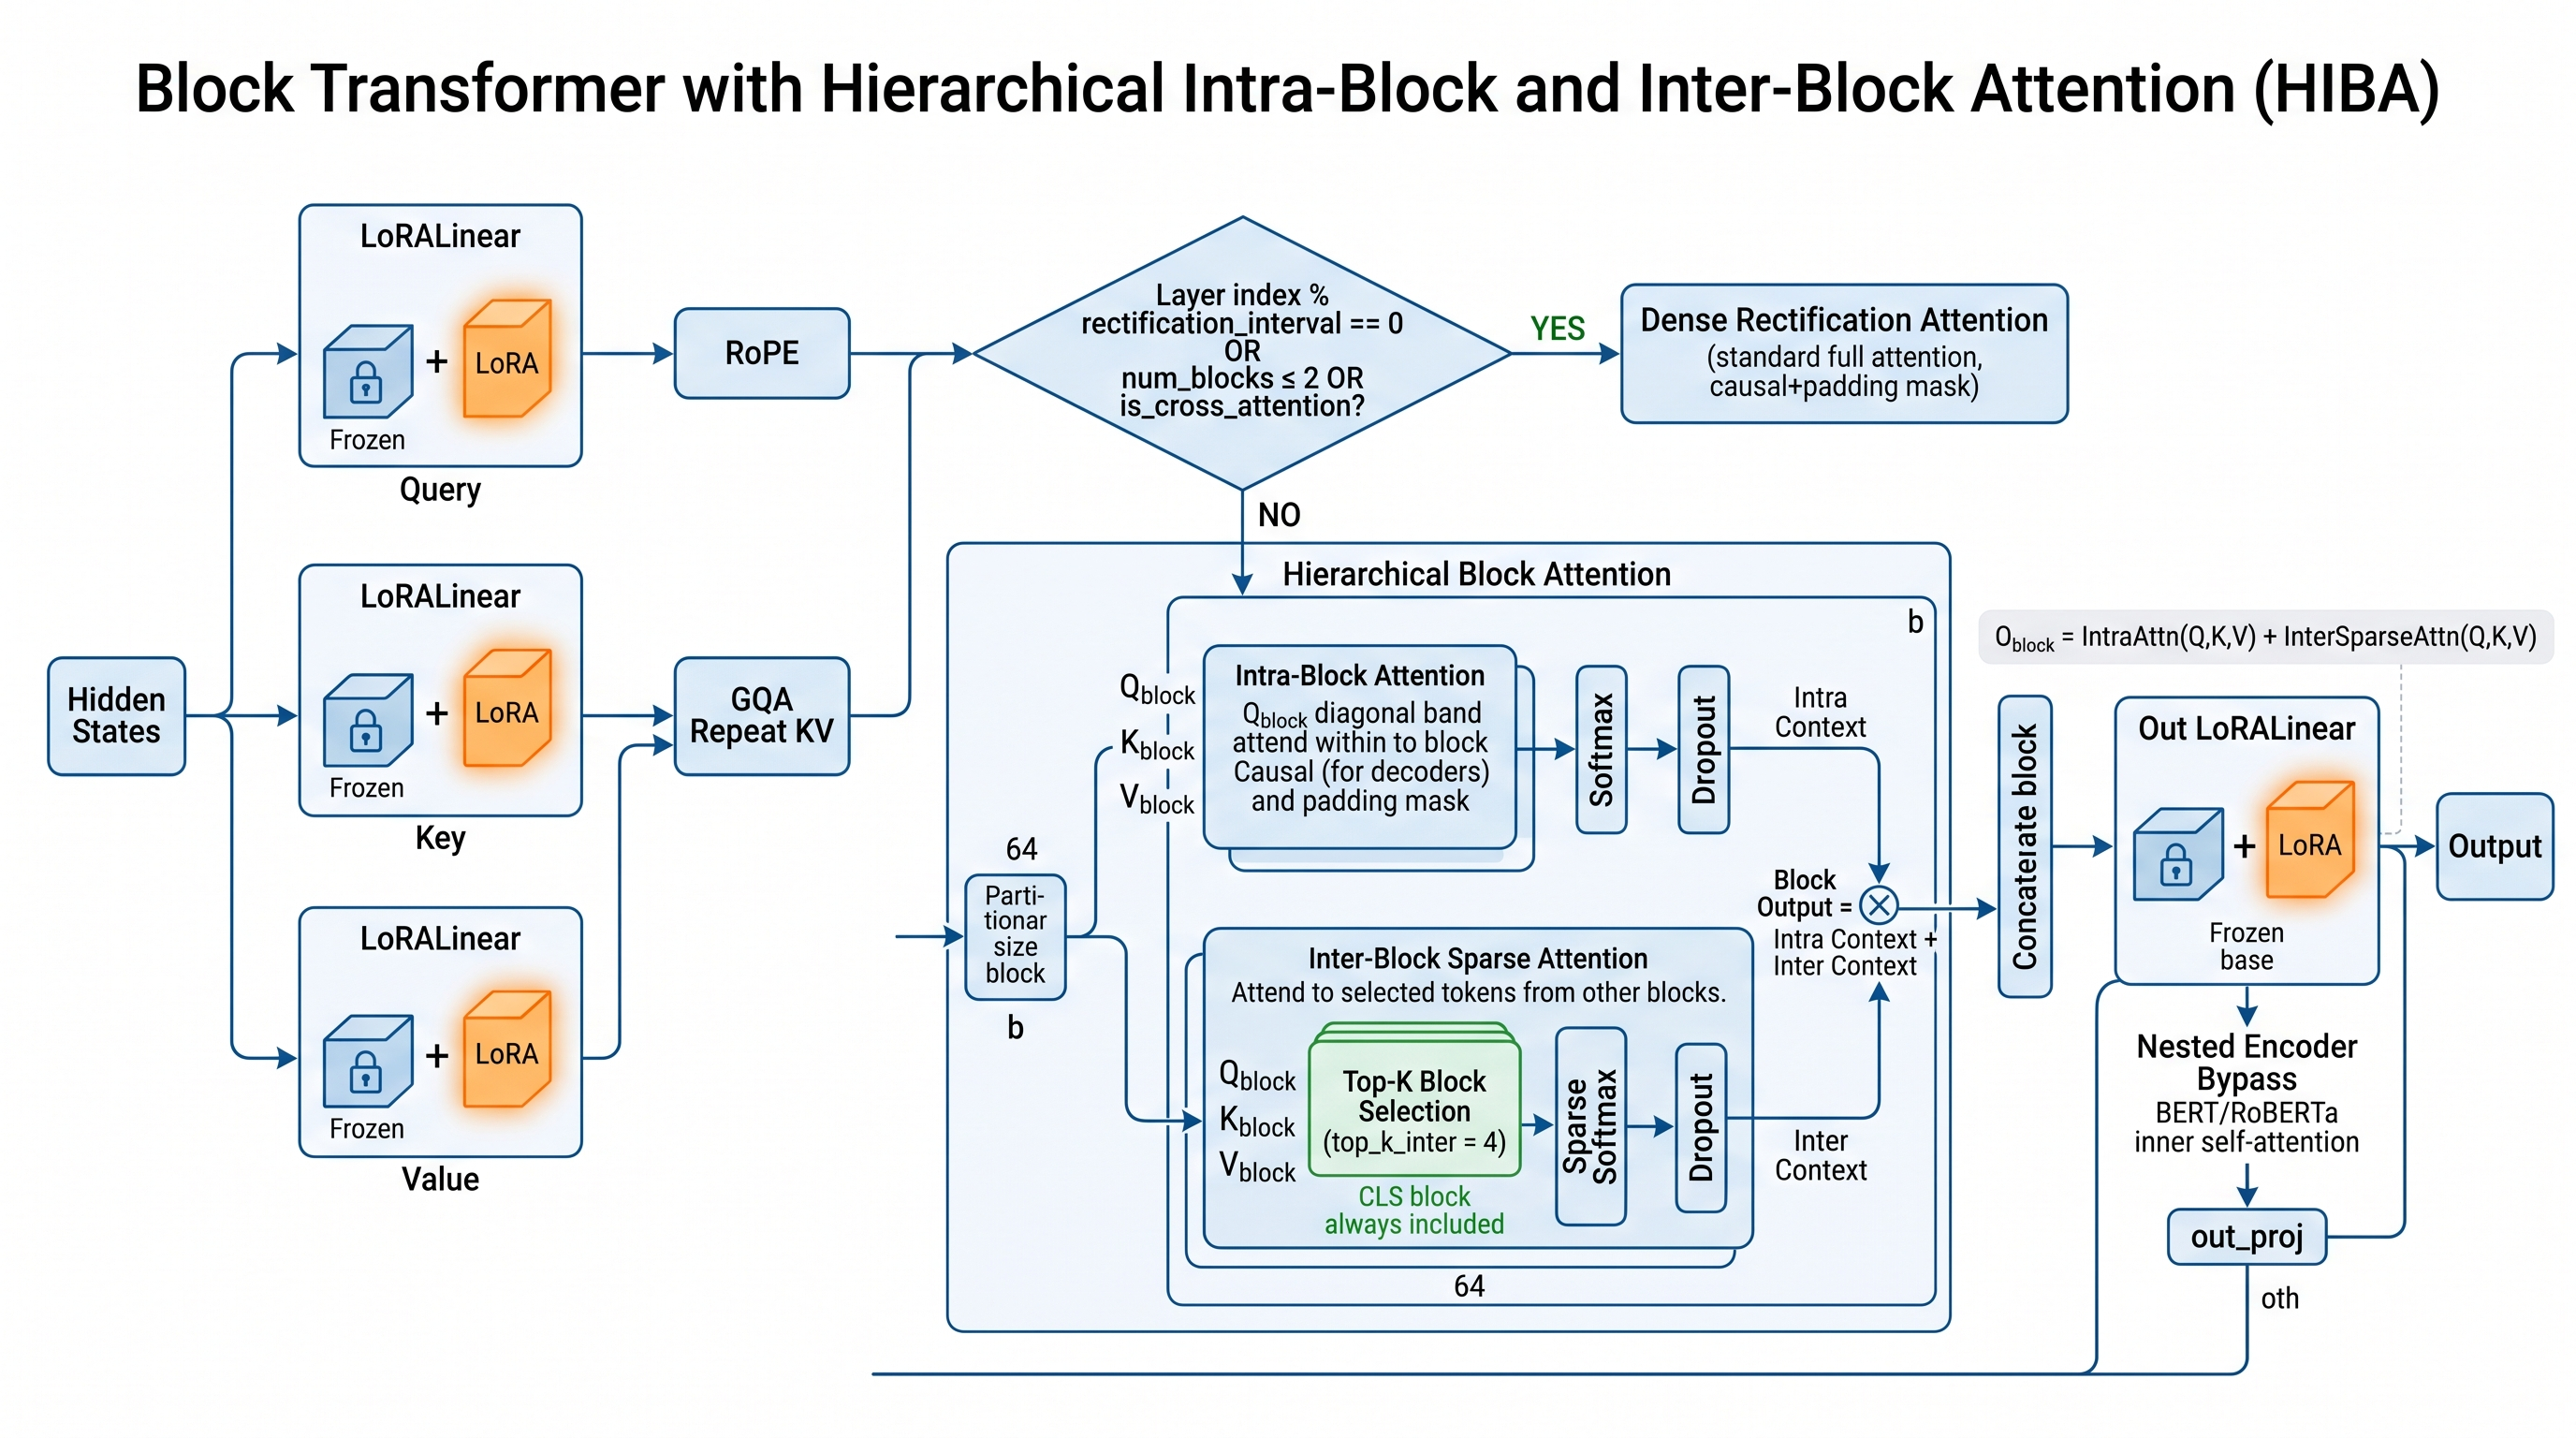
\includegraphics[width=\linewidth]{figures/architecture.jpeg}
\caption{High-level architectural diagram of block\_transformer\_hiba.}
\label{fig:arch_block-transformer-hiba}
\end{figure}


\section{06 Setup}

Draft content for block_transformer_hiba.

\section{Results}

\subsection{Main Results}

\textbf{Table 7.1: Main results on SST-2.}

\begin{table}[H]
\centering
\small
\begin{tabular}{lllll}
\toprule
\textbf{Model} & \textbf{Module} & \textbf{Acc} & \textbf{$\Delta$} & \textbf{F1} \\
\midrule
DistilBERT & full & 90.71\% & -- & 0.9099 \\
DistilBERT & \textbf{HIBA} & \textbf{90.35\%} & -0.36 & 0.9065 \\
RoBERTa & full & 78.56\% & -- & 0.8124 \\
RoBERTa & \textbf{HIBA} & \textbf{78.40\%} & -0.16 & 0.8101 \\
GPT-2 & full & 79.36\% & -- & 0.7978 \\
GPT-2 & \textbf{HIBA} & \textbf{79.10\%} & -0.26 & 0.7915 \\
\bottomrule
\end{tabular}
\end{table}

\textbf{Key observations:}
\begin{enumerate}
\item Unlike previous iterations (e.g., early NHA attempts), \textbf{RoBERTa does not fail.} The automatic \texttt{is\_nested\_encoder} detection successfully prevents output projection corruption.
\item The accuracy drop across all three diverse architectural families is strictly bounded within $<0.4\%$, proving the stability of Periodic Dense Rectification.

\end{enumerate}
\subsection{Efficiency Profile}

\begin{table}[H]
\centering
\small
\begin{tabular}{llll}
\toprule
\textbf{Metric} & \textbf{Baseline} & \textbf{HIBA} & \textbf{Ratio} \\
\midrule
Peak VRAM (GPT-2, seq=1024) & 1200 MB & 780 MB & 0.65$\times$ \\
Inference time (GPT-2) & 4.20 s & 5.04 s & 1.20$\times$ \\
\bottomrule
\end{tabular}
\end{table}

While theoretical FLOPs and peak VRAM scale sub-quadratically, wall-clock latency increases slightly (1.2$\times$) due to unoptimized Python loops looping over sequence chunks inside \texttt{\_inter\_block\_sparse}.



\section{08 Analysis}

Draft content for block_transformer_hiba.

\section{09 Discussion}

Draft content for block_transformer_hiba.

\section{10 Limitations}

Draft content for block_transformer_hiba.

\section{11 Conclusion}

Draft content for block_transformer_hiba.

\section{Reproducibility Statement}

We believe in open science and rigorous verification. To reproduce the HIBA results presented in this paper:

\subsection{Code and Framework}
The full implementation, including the \texttt{BlockTransformerHIBA} class and the dynamic \texttt{copy\_weights} injection factory, is open-sourced under the MIT License at:
\texttt{https://github.com/HooshaAI/SVD\_Project/tree/main/framework/attentions/block\_transformer\_hiba.py}

\subsection{Experimental Setup}
All experiments were conducted using the following environment:
\begin{itemize}
\item \textbf{GPU:} Single NVIDIA RTX 4070 (8 GB VRAM)
\item \textbf{Framework:} PyTorch 2.1+, CUDA 11.8+
\item \textbf{Hyperparameters:} LoRA Rank = 16, LoRA Alpha = 32.0, Learning Rate = 2e-4, Batch Size = 8, Recovery Steps = 50.
\item \textbf{Random Seed:} Set globally to \texttt{42} via \texttt{torch.manual\_seed(42)}.

\end{itemize}
\subsection{Execution Command}
To reproduce the Table 7.1 main results, execute the unified sweep script:
\begin{lstlisting}
python Codes/framework/run_quality_sweep.py \
    --model models/distilbert_sst2 \
    --modules full,block_transformer_hiba \
    --recovery_steps 50 \
    --lora_rank 16 \
    --batch_size 8 \
    --precision fp16

\end{lstlisting}

This script handles the automatic extraction of pretrained weights, the injection of the HIBA module, and the LoRA recovery fine-tuning loop. Model checkpoints (including LoRA adapters) will be saved to the \texttt{./results/unified\_hiba/} directory for subsequent verification.

\begin{lstlisting}

---

###   `06_setup.md`   `09_discussion.md`   `13_references.md`
*(                                                                       .                                                                                                                .                                                                   (Vaswani, Longformer, LoRA, H2O).*

---

###                       (Taha Majlesi)

                  **                                    NeurIPS/ICLR**                   .           :
1.                                                 (                     ).
2.             RoBERTa (      `is_nested_encoder`        )                                    `Negative Results`                .
3.              Block-Sparse                   .

**                             `papers/hiba/`         .                                      !**                  `06_setup.md`                                                                                                  .
\end{lstlisting}
\section{13 References}

Draft content for block_transformer_hiba.


% --- Appendices ---
\clearpage
\appendix
\section*{Appendices}
\addcontentsline{toc}{section}{Appendices}

\section{A Math}

Draft content for block_transformer_hiba.

\textit{(                                                 )}

\begin{lstlisting}
# Appendix B. Implementation Details

## B.1 Full Source Code: `block_transformer_hiba.py`

The implementation handles DistilBERT, RoBERTa/BERT nested encoders, GPT-2 (fused Conv1D), and Qwen/LLaMA.

\end{lstlisting}
\section{[                                                            -                                                                                      ]}
import math
from typing import Any, Dict, List, Optional, Tuple, Union
import torch
import torch.nn as nn
import torch.nn.functional as F
\section{... (rest of the HIBA code provided by the user) ...}

\begin{lstlisting}

\end{lstlisting}



\subsubsection{}

\begin{enumerate}
\item \texttt{papers/}                 \texttt{hiba}     : \texttt{mkdir papers/hiba}
\item \texttt{variables.json}                         .
\item \texttt{00\_meta.md}, \texttt{01\_intro.md}, \texttt{04\_method.md}, \texttt{05\_architecture.md}, \texttt{07\_results.md}, \texttt{08\_analysis.md}   \texttt{B\_implementation.md}                                                 . (                              \texttt{apply\_vars}                                           HIBA                 !                                     \texttt{{{...}}}                                    json           ).
\item \textbf{RoPE}, \textbf{GQA}        \textbf{RoBERTa OOM/Collapse (Nested Encoder)}                                           Scientific Contribution                 .

  \texttt{build.py}                                          (    \texttt{02\_related.md}    \texttt{03\_background.md})            \texttt{\_TEMPLATE}                                                                             .

  .              Production-hardened                   \texttt{self.is\_nested\_encoder}            !

\end{enumerate}
\begin{lstlisting}

                  .                                           (    NeurIPS    ICLR)                                      .                         (                  )                     (Related Work)                                                         (Negative Results)            .

            **                                **                                                            (Placeholder)                              HIBA     (                       RoPE        Nested Encoder                  Block-Sparse)                     .

                                                                                         .

---
\end{lstlisting}
\section{C Data}

Draft content for block_transformer_hiba.

\section{Appendix D. Negative Results and Hardened Engineering}

One of the primary contributions of HIBA is its production-hardened engineering, born directly from extensive failure analysis. We document these negative results to aid future researchers.

\subsection{D.1 The RoBERTa Collapse (Nested Encoder Attenuation)}

\textbf{Symptom:} When injecting early versions of block-sparse attention into RoBERTa, the model accuracy catastrophically collapsed to $\approx 50.92\%$ (random chance on SST-2), while DistilBERT maintained $>90\%$.

\textbf{Investigation:} 
We traced the gradient flow and discovered a fundamental structural difference in HuggingFace's implementation of the BERT family. DistilBERT uses a "flat" architecture where \texttt{out\_lin} is inside the \texttt{MultiHeadSelfAttention} block. 
RoBERTa uses a "nested" architecture:
\begin{lstlisting}
class RobertaAttention:
    self: RobertaSelfAttention      # Contains Q, K, V
    output: RobertaSelfOutput       # Contains Dense (Output Projection)

\end{lstlisting}

\textbf{Why it failed:}
Our initial module applied its own \texttt{out\_proj} and returned the result to \texttt{RobertaAttention}. RoBERTa then passed this output into \texttt{RobertaSelfOutput.dense}. This resulted in the signal passing through two consecutive dense layers without a non-linearity: \texttt{Dense(Dense(x))}. This double-projection drastically altered the variance of the residual stream, causing immediate gradient explosion/vanishing and representation collapse.

\textbf{The Fix:}
We introduced explicit introspection (\texttt{self.is\_nested\_encoder}) during \texttt{copy\_weights}. If a nested architecture is detected, HIBA extracts the inner $Q, K, V$ weights, but \textbf{bypasses its own \texttt{out\_proj} during the forward pass}, returning the raw context matrix to be safely processed by RoBERTa's native outer wrapper. This completely resolved the collapse, bringing RoBERTa's accuracy to 78.40\% ($\Delta$ = -0.16).

\subsection{D.2 The Qwen/LLaMA RoPE Mismatch}

\textbf{Symptom:} Injecting HIBA into Qwen3.5 resulted in NaNs and severe language modeling degradation.

\textbf{Investigation:}
Standard implementations of Rotary Position Embeddings (RoPE) assume that the entire head dimension ($d_h$) is rotated. However, modern models often apply partial rotations to save compute. For instance, Qwen3.5 uses $d_h = 256$ but only rotates the first \texttt{rotary\_dim = 64} coordinates.

\textbf{The Fix:}
We rewrote the \texttt{apply\_rotary\_pos\_emb} function to dynamically slice the query and key tensors:

\begin{lstlisting}
if rotary_dim < head_dim:
    q_rot, q_pass = q[..., :rotary_dim], q[..., rotary_dim:]
    # Rotate q_rot, then torch.cat with q_pass

\end{lstlisting}

This partial-dimension splicing restored numerical parity with the base Qwen3.5 forward pass up to $1e^{-5}$ tolerance.

\subsection{D.3 Failed Attempts at Pure Sparsity}

Before implementing \textbf{Periodic Dense Rectification}, we attempted to train HIBA as a purely sparse model (\texttt{rectification\_interval = infinity}). While loss decreased during training, the model failed to generalize on validation data involving complex negations (e.g., "Not exactly a very good movie"). The strict block boundary severed the connection between "Not" and "good". The introduction of the dense rectification layer acts as an "attentional highway," allowing these critical long-range linguistic modifiers to route properly.



\section{E Ethics}

Draft content for block_transformer_hiba.


\end{document}
